\section{Economic Production Quantity}

\Opensolutionfile{ans}

\label{sec:finite-prod-rates}

\begin{exercise}
 Suppose that the delivery rate of the items we order is not
 `infinite', as it is in the EOQ setting (recall, in the EOQ we
 assume instantaneous deliveries). If we have a machine that
 replenishes the FGI we have to take into account the production
 rate, $r$ say. If it costs $K$ to switch on the machine, when do you switch the machine on or off?
 \begin{solution}
   An easy policy is to switch the machine on when the FGI level hits
   some level $Q$, and switch it off when the level is $0$. Of course
   we need to assume that $D<r$, i.e., the production rate is larger
   than the demand rate $D$. 

   To find an expression to cover this situation we can reason like
   this.  When the machine is on, inventory increases at rate
   $r-D$. If we keep it on for $T$ time units, then the inventory
   level is $T(r-D)$ when we switch off. The time until the inventory
   hits 0 is then $T(r-D)/D$, since we start with an inventory level
   $T(r-D)$ after switching off and the demand rate is $D$. Thus, the total cycle length is
   \begin{equation*}
     T + \frac{T(r-D)}D = T + T(\frac{r}D-1) = T + T\frac r D - T = T\frac r D.
   \end{equation*}

   What is, in the EOQ, the average inventory cost? It is half the
   maximal height times $h$, i.e., $hQ/2$. In our present case, the
   maximal height is $T(r-D)$. Thus the average inventory cost must
   be  $hT(r-D)/2$. 

   The ordering cost in the EOQ is $A$ times the order frequency, i.e., $A D/Q$. Here the time between two `order' moments (switching moments) is $Tr/D$. Hence, the frequency is $D/rT$ and the average switching cost is $K D/rT$. 

All in all we get for the average cost
\begin{equation*}
 \frac{h(r-D)}2 T + \frac{K}r \frac DT.
\end{equation*}
This is similar to the EOQ model with $h'=h(r-D)$ and $A=K/r$. But then the optimal $T$ must be given by
\begin{equation*}
 T = \sqrt{\frac{2AD}{h'}} = \sqrt{\frac{2DK/r}{h(r-D)}}=\sqrt{\frac{2DK}{hr(r-D)}}.
\end{equation*}
 \end{solution}
\end{exercise}

  

\begin{exercise}
We have thus far only considered environments where inventories are replenished from an external source. Does the EOQ model apply to production environments?


\begin{solution}
It does. This version of the EOQ is often referred to as the EPQ (Economic Production Quantity) model. The difference between EOQ and EPQ models lies in how they treat replenishments:
\begin{enumerate}
\item The EOQ model assumes that the order arrive all at once.
\item The EPQ model assumes that once production is switched on items are produced on a continuous basis with a fixed rate.
\end{enumerate}
\end{solution}
\end{exercise}

\begin{exercise}
Explain the inventory policy behind the EPQ model. What are its parameters? How does it work?


\begin{solution}
The policy works as follows. We switch on production when the inventory level hits zero. Then we produce $Q$ units and then we switch off. The policy thus have a single parameter $Q$, i.e. production quantity in one replenishment cycle. 
\end{solution}
\end{exercise}

\begin{exercise}
Illustrate how the inventory behaves over time for the EPQ model. Then write down the cost function and characterize the optimal policy parameters.


\begin{solution}

See Figure~\ref{fig:EPQ}.

\begin{figure}[htbp]
\centering
\small
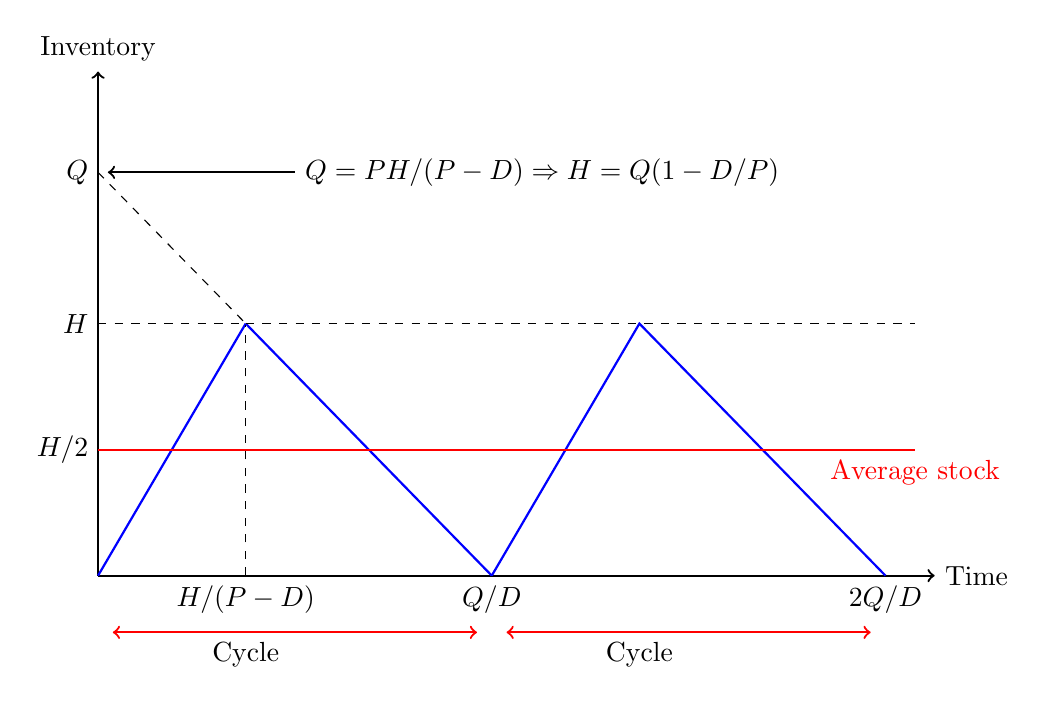
\begin{tikzpicture}[x=1.25cm,y=0.016cm]
\draw[thick,->] (0,0) -- (8.5,0) node[right] {Time};
\draw[thick,->] (0,0) -- (0,400) node[above] {Inventory};
\draw[] (0,200) node[left] {$H$};
\draw[dashed] (0,200) -- (1.5,200);
\draw[color=blue,thick] (0,0) -- (1.5,200);
\draw[] (1.5,0) node[below] {$H / (P-D)$};
\draw[dashed] (1.5,0) -- (1.5,200);
\draw[color=blue,thick] (1.5,200) -- (4,0);
\draw[dashed] (0,4*200/2.5) -- (1.5,200);
\draw[] (0,4*200/2.5) node[left] {$Q$};
\draw[] (4,0) node[below] {$Q / D$};
\draw[thick,<-] (0.1,4*200/2.5) -- (2,4*200/2.5) node[right] {$Q = PH / (P - D) \Rightarrow  H = Q(1 - D / P)$};
\draw[dashed] (1.5,200) -- (8.3,200);
\draw[color=blue,thick] (4,0) -- (4+1.5,200) -- (8,0);
\draw[] (8,0) node[below] {$2Q / D$};
\draw[] (0,100) node[left] {$H / 2$};
\draw[color=red,thick] (0,100) -- (8.3,100) node[below] {Average stock};
\foreach \y in {0,...,1}{
	\draw[color=red,thick,<->] (4*\y+0.15,-45) -- (4*\y+4-0.15,-45);
	\draw[] (4*\y+1.5,-45) node[below] {Cycle};}
\end{tikzpicture}
\caption{EPQ model}
\label{fig:EPQ}
\end{figure}

It is important to observe that the inventory behaves differently when production is on and off. If production is on, then the inventory increases with the rate $P-D$. Here $P$ stands for the production rate i.e. number of items produced in unit time. Note that $P$ is supposed to be larger than $D$, as it would otherwise be impossible to cover the demand. If production is off, the inventory process is the same with the classical model where it decreases with rate $D$. The production quantity in one cycle is $Q$. At the beginning of each cycle, production is switched on and it is switched off once $Q$ items have been produced. Because the inventories increase with rate $P-D$ during that time, we end up with $H=Q(1-\frac{D}{P})$ units once the machine has been turned off. Then production remains off until the inventory level drops down to zero, and then another cycle starts.

The total cost for one cycle is the sum of ordering cost, procurement cost, and inventory (holding) cost. The fixed setup cost (rather than fixed ordering) is $A$ per cycle as we switch on the machine only once in each cycle. The production cost (rather than procurement) equals the unit production cost times the order quantity $cQ$, i.e. we produce just enough to satisfy all the demand in each cycle. The inventory cost per cycle is the total area of the triangle times $h$, i.e. 
\begin{equation*}
h~\frac{\text{height}\cdot\text{base}}{2} = h~\frac{H \cdot Q/D }{2} = \left(1-\frac{D}{P}\right) \frac{h Q^2}{2D}.
\end{equation*}

Thus, the total cycle cost is $A+cQ+\frac{(1-\frac{D}{P}) h Q^2}{2D}$. The average cost per unit time is this total cost divided by the duration of one cycle, which is $\frac{Q}{D}$. Therefore, the average cost is
\begin{equation*}
A \frac{D}{Q}+cQ \frac{D}{Q} + \left(1-\frac{D}{P}\right) \frac{h Q^2}{2D} \frac{D}{Q} = \frac{AD}{Q}+cD+\left(1-\frac{D}{P}\right)\frac{hQ}{2}
\end{equation*}

This expression gives us the average cost as a function of the order quantity:
\begin{equation*}
f(Q) = \frac{AD}{Q}+cD+\left(1-\frac{D}{P}\right)\frac{hQ}{2}.
\end{equation*}

It is easy to observe at this point that we can derive the average cost function of the EPQ model simply by revising the holding cost $h$ of the EOQ model as $h'=h \left(1-\frac{D}{P}\right)$. All relevant results, such as expressions of the optimal order quantity and cost then immediately follows. For instance, the optimal production quantity $Q^*=\sqrt{\frac{2AD}{h'}}$ and optimal average cost per unit time $f(Q^*)=\sqrt{2ADh'}+cD$. The intuition behind is as follows. Let us assume that we are using the same $Q$ for the EOQ and EPQ models. Then the average stock level and thus the holding costs of the EPQ model will be $1-\frac{D}{P}$ times the average stock level of the EOQ model, and all other costs will be the same.  
\end{solution}
\end{exercise}

\begin{exercise}
For which parameter settings the optimal policies EOQ and EPQ models have a similar structure? 


\begin{solution}
Recall that the main difference between EOQ and EPQ models is that EOQ assumes the order arrive all at once and EPQ assumes items are produced with a fixed rate. Let us consider the EPQ model and assume that the production rate is extremely high. Then production becomes almost instantaneous. This setting should yield the same results with the EOQ model.

This is obvious if we look at the average cost function $f(Q) = \frac{AD}{Q}+cD+\frac{h'Q}{2}$ where $h'=h\left(1-\frac{D}{P}\right)$. If $P$ is very large, then 
$\left(1-\frac{D}{P}\right)$ approaches 1. Then $h'\approx h$ and we have the same cost function. For moderate values of $P$ the expression $\left(1-\frac{D}{P}\right)$ will be in between 0 and 1. Then $h'<h$ and it implies that the EPQ function is lower than the EOQ function.
\end{solution}
\end{exercise}

\begin{exercise}
How does the production rate affect the optimal production quantity and the average cost per unit time?


\begin{solution}
Let us consider the optimal production quantity $Q^*=\sqrt{\frac{2AD}{h'}}$ and corresponding optimal average cost per unit time $f(Q^*)=\sqrt{2ADh'}+cD$ where $h'=h\left(1-\frac{D}{P}\right)$. It is clear that the smaller the $P$ the smaller the adapted holding cost $h$. Then it is easy to see that a higher production rate leads to a smaller $Q^*$ and a higher $f(Q^*)$. 

We know that the production rate should be larger than the demand rate to be able to cover demand over time. Thus, the lowest feasible production rate is the demand rate itself. In this case we have $P=D$ and therefore $h'=h\left(1-\frac{D}{D}\right)=0$. The mathematics of this particular case is ill-defined to the division by 0. Nevertheless, it is easy to see what is going on. Because the production rate equals the demand rate; we simply have is no inventory! We switch on the machine and leave it switched on all the time. Thus we have neither fixed setup cost nor holding cost. All we need to pay is the production cost which is $cD$ per unit time.
\end{solution}
\end{exercise}

\begin{exercise}
It appears that having a slower production rate is favorable. How does this makes sense?

\begin{solution}
The issue is with the trade-off between setup and holding costs. If the machine is fast, then once you switch on you quickly build up inventories at a high speed. To avoid excessive inventories you switch off. But then you pay the setup cost more frequently. 
\end{solution}
\end{exercise}



\Closesolutionfile{ans}
\opt{solutionfiles}{
\subsection{Solutions}
\input{ans}
}

\clearpage

%%% Local Variables:
%%% mode: latex
%%% TeX-master: "inventory_notes"
%%% End:
